\documentclass[8pt]{beamer}
\usepackage[nobglogo]{beamerthemedmi-owled}
\usepackage[utf8x]{inputenc}
\usepackage{default}
\usepackage{url}
\usepackage{verbatim}
\usepackage{graphicx}
\usepackage{mathrsfs}
\usepackage{dl}
\usepackage{mls}
\usepackage{fancyvrb}
%\usepackage{listings}


\mode<presentation>
{
  \usetheme{dmi-owled}
  %\usetheme{Warsaw}
  % or ...

  \setbeamercovered{transparent}
  % or whatever (possibly just delete it)
}

\title{Linked Open Data e Semantic Web:\\
Fondamenti e Linguaggi di Interrogazione\\
Parte Seconda}

\author{Cristiano Longo\\ 
{\small{longo@dmi.unict.it}}}



\date{Universit\`a di Catania, 11/10/2014}
\newcommand{\urlsingle}[1]{{\small {\center {\url{#1}}}}}
\begin{document}
\maketitle
\setcounter{tocdepth}{1}

\newcommand{\CNames}{N_C}
\newcommand{\PNames}{N_P}
\newcommand{\INames}{N_I}
\newcommand{\VNames}{V}
\newcommand{\DNames}{N_D}
\newcommand{\LNames}{N_L}
\newcommand{\BlankNodes}{\mathcal{B}}
\newcommand{\IRI}{IRI}


%\newcommand{\StringT}{\mathtt{String}}
\newcommand{\Ont}{\mathcal{O}}
\newcommand{\Ontp}{\mathcal{O'}}

\newcommand{\datatypes}{\mathcal{D}}
%\newcommand{\literal}[2]{"#1"\hat{ }\hat{ }#2} % TODO
%\newcommand{\literal}[2]{\mbox{"#1"#2}} % TODO
\newcommand{\stringLiteral}[1]{\mbox{``#1''}}
\newcommand{\literal}[2]{\mbox{``#1''\textasciicircum\textasciicircum\url{#2}}} % TODO
\newcommand{\literals}{\mathcal{L}}
\newcommand{\Vocab}{\mathcal{V}}

\section{Ontologie}

\begin{frame}
 \frametitle{Ontologie - Sintassi}

Siano $\CNames$, $\PNames$, $\INames$ tre insiemi infiniti, numerabili e 
a due a due disgiunti di nomi di \emph{classe}, \emph{propriet\`a} e \emph{individuo},
rispettivamente.
\vspace{\baselineskip}

Una \emph{ontologia} \`e un insieme finito di asserzioni dei seguenti tipi:
\[
 \begin{array}{ll}
  \mbox{(Constraints)} & C \Issub D\\
  & P \Issub Q \\
  & \dom(P) \Issub C \\
  & \range(P) \Issub C \\
  &\\
  \mbox{(Class Assertions)} & C(a)\\
  &\\
  \mbox{Property Assertions} & a\,P\,b\;(\mbox{equivalente }P(a,b))\\
 \end{array}
\]
dove $C, D \in \CNames$, $P, Q \in \PNames$ e $a, b \in \INames$.
\end{frame}

\begin{frame}
 \frametitle{Ontologie - Semantica}
Una \emph{interpretazione} $\I=(\Delta^{\I}, \cdot^{\I})$ \`e una coppia
$\Delta^{\I}$, $\cdot^{\I}$ dove:
\begin{itemize}
 \item $\Delta^{\I}$ \`e un insieme non vuoto;
 \item $\cdot^{\I}$ \`e una funzione (polimorfa) che associa
 \begin{itemize}
  \item ad ogni nome di concetto $C$ in $\CNames$ un sottoinsieme $C^{\I}$ di
  $\Delta^{\I}$,
  \item ad ogni nome di propriet\`a in $P$ in $\PNames$ una relazione $P^{\I}$su
  $\Delta^{\I}$,
  \item ad ogni nome di individuo $a$ in $\INames$ un elemento $a^{\I}$ di
  $\Delta^{\I}$.
 \end{itemize}
\end{itemize}

\uncover<2->{
La nozione di \emph{soddisfacibilit\`a} \`e definita come segue ($\I \models
\alpha$ si legge $\I$ soddisfa $\alpha$):
\[
\begin{array}{ccl}
 \I\models C \Issub D & \Longleftrightarrow & C^{\I} \subseteq D^{\I}\\  
 \I\models P \Issub Q & \Longleftrightarrow & P^{\I} \subseteq Q^{\I}\\  
 \I\models \dom(P) \Issub C & \Longleftrightarrow & (\forall [x,y] \in P^{\I})(x
 \in C^{\I})\\
 \I\models \range(P) \Issub C & \Longleftrightarrow & (\forall [x,y] \in
 P^{\I})(y \in C^{\I})\\
 \I\models C(a) & \Longleftrightarrow & a^{\I} \in C^{\I}\\  
 \I\models a\,P\,b & \Longleftrightarrow & [a^{\I}, b^{\I}] \in P^{\I}
\end{array} 
\]
per ogni $C, D \in \CNames$, $P, Q \in PNames$, $a,b \in \INames$.
\vspace{\baselineskip}

}
\uncover<3->{
Sia $\Ont=\{\alpha_1, \ldots, \alpha_n\}$ una ontologia. 
\[
\I \models \Ont \iff \I \models \alpha_i\mbox{ per ogni }1\leq i\leq n .
\]
}
\uncover<4->{
Siano $\Ont$ e $\Ontp$ due ontologie. $\Ont$ \emph{implica} $\Ontp$ sse
\[
\I \models \Ont \Longrightarrow \I \models \Ontp
\]
per ogni possibile interpretazione $\I$.
}
\end{frame}

\begin{frame}
\frametitle{Ontologie nel Web Semantico}

Le ontologie definite usando tecnologie del Web Semantico hanno particolari
caratteristiche:

\begin{itemize}[<+->]
	\item tutti i \emph{nomi} sono degli \emph{Internationalized Resource
	Identifier (IRI))}, ossia
\[
 \CNames \cup \PNames \cup \INames \subseteq IRI ;
\]
  \item possono contenere dei \emph{letterali}, che vengono usati per
  rappresentare tipi di dato \emph{concreti} (ad esempio stringhe di testo, numeri, date,
  \ldots).
\end{itemize}

\end{frame}

\begin{frame}
\frametitle{International Resource Identifier}

La specifica \emph{International Resource Identifier} (in breve \emph{IRI},
vedi RFC3987) estende quella per gli \emph{Uniform Resource Identifier} (in breve \emph{URI},
vedi RFC3986) con un pi\`u ampio repertorio di caratteri, aggiungendo
funzionalit\`a per l'internazionalizzazione.
\vspace{\baselineskip}

Nel seguito indicheremo con $\IRI$ l'insieme di tutti
i possibili IRI (i.e. l'insieme delle stringhe che rispettano la 
specifica IRI).
\end{frame}

\begin{frame}
\frametitle{IRI nel Web Semantico}
Nell'ambito del Web Semantico, tutti gli oggetti reali o concreti sono
identificati attraverso IRI. As esempio
\begin{center}
 \url{http://dbpedia.org/resource/Leonardo_da_Vinci}
\end{center}
\`e la IRI usata nell'ontologia \url{dbpedia.org} per indicare
Leonardo da Vinci, e ancora 
\begin{center}
  \begin{small}
    \url{http://data.europeana.eu/item/04802/243FA8618938F4117025F17A8B813C5F9AA4D619}
  \end{small}
\end{center}
indica la \emph{Mona Lisa} nell'ontologia del progetto \emph{Europeana}.
\end{frame}

\begin{frame}
\frametitle{IRI nel Web Semantico - \emph{Sinonimie}}
Si noti che una IRI \`e associata ad un unico oggetto, ma ad 
ogni oggetto possono essere associati diversi IRI.
\vspace{\baselineskip}

Ad esempio le seguenti IRI sono entrambe associate alla Monnalisa:
\vspace{\baselineskip}

\begin{small}
  \begin{tabular}{l}
      \url{http://data.europeana.eu/item/04802/243FA8618938F4117025F17A8B813C5F9AA4D619}\\
    \\
      \url{http://dbpedia.org/page/Mona_Lisa} .
  \end{tabular}
\end{small}
\end{frame}

\begin{frame}
  \frametitle{IRI nel Web Semantico - Namespaces}
  
  Nelle ontologie del Web Semantico le IRI possono essere abbreviate
  con il meccanismo dei \emph{namespace} (prefissi), mutuato da XML.
  \vspace{\baselineskip}
  
\uncover<2->{
  Ad ogni ontologia spesso \`e assegnato un \emph{base prefix}.
  Viene usato come prefisso per ottenere le IRI complete degli oggetti
  dell'ontologia nel caso in cui la IRI specificata sia \emph{incompleta}. Ad
  esempio, se il base prefix dell'ontologia $\Ont$ \`e \url{http://example.org/},
  \[
   Alice \quad \Longrightarrow \mathtt{http://example.org/Alice} . 
  \]
}  

\uncover<3->{
  \`E possibile specificare degli ulteriori \emph{prefix}
  come coppie
  \[
   <prefix name> \quad \longrightarrow \quad <prefix uri> 
  \]
  e \emph{abbreviare} delle IRI nell'ontologia con la
  sintassi $<prefix name>:<IRI specific part>$. 
  \vspace{\baselineskip}
  
  Se ad
  esempio nell'ontologia \`e definito il prefisso
  \[
   ex2 \quad \longrightarrow \quad \mathtt{http://example2.org/}
  \]
  la IRI \url{ex2:Alice} verr\`a espansa in
  \url{http://example2.org/Alice} .
}
\end{frame}

\begin{frame}
\frametitle{Letterali}

I letterali vengono usati per rappresentare tipi di dato \emph{concreti},
come ad esempio stringhe di testo, numeri, date, \ldots
\vspace{\baselineskip}

Grazie ai letterali \`e possibile ad esempio esprimere affermazioni dei seguenti tipi:
\begin{itemize}
 \item Il cognome di Mario \`e \emph{Rossi};
 \item Cristiano \`e nato il giorno \emph{22 Marzo 1979};
 \item L'Empire State Building \`e alto \emph{380 metri}.
\end{itemize}
\end{frame}

\begin{frame}
\frametitle{Datatype}
Per introdurre i Letterali \`e necessario fornire prima la definizione di \emph{datatype}
(vedi \url{http://www.w3.org/TR/2014/REC-rdf11-concepts-20140225/\#section-Datatypes} e 
\url{http://www.w3.org/TR/xmlschema11-2/}).
\vspace{\baselineskip}

Un \emph{datatype} \`e caratterizzato da tre componenti:
\begin{itemize}
 \item un \emph{lexical space}, ossia un insieme di stringhe (finite) di caratteri nella codifica \emph{UNICODE};
 \item un \emph{value space}, che \`e un insieme non meglio specificato e numerabile di \emph{valori} (interi, date,
 Booleani, \ldots);
 \item un \emph{lexical-value mapping} che associa ad ogni stringa nel lexical space un elemento nel value space.
\end{itemize}
\vspace{\baselineskip}

I datatype vengono di solito indicati con delle IRI.
\end{frame}

\begin{frame}
\frametitle{Datatype - Esempio 1 : \url{xsd:integer}}
Il datatype \url{xsd:integer} (dove \url{xsd} \`e l'abbreviazione per il namespace \url{http://www.w3.org/2001/XMLSchema\#})
\`e definito come segue:

\begin{itemize}
 \item il \emph{lexical space} di \url{xsd:integer} \`e costituito da tutte le sequenze finite di cifre da 0 a 9, possibilmente
 precedute dal carattere ``-'' o ``+'';
 \item il \emph{value space} \`e l'insieme dei numeri interi;
 \item il valore di una stringa nel lexical space di \url{xsd:integer} si ottiene considerando le cifre 
 presenti nella stringa come cifre del corrispondente numero in base $10$, e moltiplicando il numero cos\`i ottenuto per
 $-1$ nel caso in cui la stringa inizi con il carattere ``-''.
\end{itemize}
\end{frame}

\begin{frame}
\frametitle{Datatype - Esempio 2 : \url{xsd:string}}
Il datatype \url{xsd:string} \`e definito come segue:

\begin{itemize}
 \item il \emph{lexical space} di \url{xsd:string} comprende 
 tutte le sequenze di caratteri (UNICODE) di zero o pi\`u caratteri;
 \item il \emph{value space} di \url{xsd:string} coincide col suo 
 lexical space;
 \item il \emph{lexical-value mapping} associa ogni stringa nel lexical space
 con se stessa (indetit\`a).
 \end{itemize}
\end{frame}

\begin{frame}
 \frametitle{Altri esempi di datatype}
Riportiamo alcuni datatype (mutuati da XML Schema) di uso comune.

\begin{small}
\begin{tabular}{|l|l|}
 \hline
\url{xsd:boolean} & true, false\\
\url{xsd:decimal} & Arbitrary-precision decimal numbers\\
\url{xsd:integer} & Arbitrary-size integer numbers\\
\url{xsd:double} & 64-bit floating point numbers incl. ±Inf, ±0, NaN\\
\url{xsd:float} & 32-bit floating point numbers incl. ±Inf, ±0, NaN\\
\url{xsd:date} & Dates (yyyy-mm-dd) with or without timezone\\
\url{xsd:time} & Times (hh:mm:ss.sss…) with or without timezone\\
\url{xsd:dateTime} & Date and time with or without timezone\\
\url{xsd:dateTimeStamp} & Date and time with required timezone\\
\url{xsd:duration} & Duration of time\\
\url{xsd:byte} & -128\ldots+127 (8 bit)\\
\url{xsd:short} & -32768\ldots+32767 (16 bit) \\
\url{xsd:int} & -2147483648\ldots+2147483647 (32 bit)\\
\url{xsd:long} & -9223372036854775808\ldots+9223372036854775807 (64 bit)\\
\url{xsd:unsignedByte} & 0\ldots255 (8 bit)\\
\url{xsd:unsignedShort} & 0\ldots65535 (16 bit)\\
\url{xsd:unsignedInt} & 0\ldots4294967295 (32 bit)\\
\url{xsd:unsignedLong} & 0\ldots18446744073709551615 (64 bit)\\
\url{xsd:positiveInteger} & Integer numbers $>0$\\
\url{xsd:nonNegativeInteger} & Integer numbers $\geq 0$\\
\url{xsd:negativeInteger} & Integer numbers $<0$\\
\url{xsd:nonPositiveInteger} & Integer numbers $\leq 0$\\
\url{xsd:hexBinary} & Hex-encoded binary data\\
\hline
\end{tabular}
\end{small}
\end{frame}

\begin{frame}
\frametitle{Letterali - Definizione}
Formalmente, i letterali sono definiti come segue (vedi 
\url{http://www.w3.org/TR/2014/REC-rdf11-concepts-20140225/\#section-Graph-Literal}).
\vspace{\baselineskip}

Un \emph{letterale} \`e costituito da un \emph{datatype} $t$ e da una 
stringa di caratteri nel lexical space di $t$ (la cosiddetta \emph{lexical form}
del letterale).
\vspace{\baselineskip}

Se un letterale \`e di tipo \url{xsd:string}, ad esso pu\`o essere associato un
\emph{language tag} ad indicarne la \emph{lingua}. Per i valori che questo attributo pu\`o
assumere fare riferimento allo \emph{IANA Language Subtag Registry}.
\end{frame}

\begin{frame}
\frametitle{Letterali - Esempi}
Seguono alcuni esempi di letterali:

\begin{center}
\begin{tabular}{|l|l|c|}
  \hline
  \textbf{lexical form} & \textbf{data type} & \textbf{language tag}\\
  \hline
  ``380'' & \url{xsd:integer} & - \\
  ``March-22-1979'' & \url{xsd:date} & - \\
  ``Rossi'' & \url{xsd:string} & - \\
  ``Parigi'' & \url{xsd:string} & it \\
  ``Paris'' & \url{xsd:string} & en\\
  \hline
\end{tabular}
\end{center}
\vspace{\baselineskip}

Nel caso in cui si ometta l'indicazione del tipo di dato, il letterale si assume essere
di tipo \url{xsd:string}.
\end{frame}


\begin{frame}
\frametitle{Letterali - Notazione (1/3)}
Per indicare i letterali spesso si usano le seguenti notazioni
\[
 \begin{array}{c}
   \literal{lexform}{type} \\
   \\
  < lexform, type >
 \end{array}
\]
ove $lexform$ e $type$ sono la lexical form e il data type del letterale, rispettivamente.
\vspace{\baselineskip}

Alcuni esempi:
\[
\begin{array}{ll}
 \literal{380}{xsd:integer} & <``380'', \mathtt{xsd:integer}>\\
 \literal{March-22-1979}{xsd:date} & <``March-22-1979'', \mathtt{xsd:date}>\\
 \literal{Rossi}{xsd:string} & <``Rossi'', \mathtt{xsd:string}>
\end{array}
\]
\end{frame}

\newcommand{\mathurl}[1]{\mbox{\url{#1}}}

\begin{frame}
\frametitle{Letterali - Notazione (3/3)}
Dato un letterale $l$, indicheremo con
\begin{itemize}
 \item $datatype(l)$ il tipo di dato di $l$, e con 
 \item $lexform(l)$ la lexical form di $l$.
\end{itemize}
\vspace{\baselineskip}

Seguono alcuni esempi:
\[
\begin{array}{l}
 datatype(\literal{380}{xsd:integer}) = \mathurl{xsd:integer}\\
 datatype(\literal{March-22-1979}{xsd:date}) = \mathurl{xsd:date}\\
 datatype(\literal{Rossi}{xsd:string}) = \mathurl{xsd:string}\\
 \\
 lexform(\literal{380}{xsd:integer}) = \stringLiteral{380}\\
 lexform(\literal{March-22-1979}{xsd:date}) = \stringLiteral{March-22-1979}\\
 lexform(\literal{Rossi}{xsd:string}) = \stringLiteral{Rossi} 
\end{array}
\]
\end{frame}


\begin{frame}
\frametitle{Confronto tra Letterali}
Due letterali sono uguali se e solo se sono uguali le loro lexical form,
se hanno lo stesso tipo e se sono uguali i loro language tag, ove presenti.
Di conseguenza due letterali possono essere diversi anche avendo lo stesso
\emph{valore}. Ad esempio i due seguenti letterali hanno entrambi 
come valore l'intero $1$ ma sono diversi:
\vspace{\baselineskip}

\[
 \begin{array}{l}
  \literal{1}{xsd:integer}\\
  \literal{01}{xsd:integer} .\\
 \end{array}
\]
\end{frame}

\begin{frame}
\frametitle{Property Assertions con Letterali}

I letterali possono essere usati per specificare \emph{propriet\`a} di un
individuo. In altre parole, essi possono comparire come \emph{oggetto}
di una property assertion. Alcuni esempi di role assertion che coinvolgono
letterali sono
\[
 \begin{array}{l}
  Mario \, surname \, \literal{Rossi}{xsd:string} \\
  Cristiano \, hasbirth \, \literal{March-22-1979}{xsd:date}\\
 \end{array}
\]
con $Mario, Cristiano \in \INames$, $surname, hasbirth \in \PNames$ e 
$\literal{Rossi}{xsd:string}$, $\literal{March-22-1979}{xsd:date}$ letterali.

\end{frame}

\begin{frame}
 \frametitle{Ontologie nel Web Semantico - Sintassi}

Siano $\CNames$, $\PNames$, $\INames$, $\DNames$, $\literals$ insiemi
infiniti, numerabili e a due a due disgiunti di nomi di \emph{classe}, \emph{propriet\`a},
\emph{individuo} e di  \emph{datatype} e di \emph{letterali}, rispettivamente,
tali che
\[
	\CNames \cup \PNames \cup \INames \cup \DNames \subseteq \IRI , 
\]
e $\literals$ siano i letterali (nel senso visto prima) i cui datatype
sono in $\DNames$.

Una \emph{ontologia} \`e un insieme finito di asserzioni dei seguenti tipi:
\[
 \begin{array}{ll}
  \mbox{(Constraints)} & C \Issub D\\
  & P \Issub Q \\
  & \dom(P) \Issub C \\
  & \range(P) \Issub C \\
  &\\
  \mbox{(Class Assertions)} & C(a)\\
  &\\
  \mbox{Property Assertions} & a\,P\,b\\
  & \mathbf{a\,P\,l}\\
 \end{array}
\]
dove $C, D \in \CNames$, $P, Q \in \PNames$, $a, b \in \INames$,
e $l \in \LNames$.
\end{frame}

\begin{frame}
 \frametitle{Ontologie nel Web Semantico - Semantica}
Una \emph{interpretazione} \`e una
tripla $\I=(\Delta^{\I}$, $\Delta_{D}^{\I}$, $\cdot^{\I})$ dove:
\begin{itemize}
 \item $\Delta^{\I}, \Delta_{D}^{\I}$ sono due insiemi disgiunti e non vuoti;
 \item $\cdot^{\I}$ \`e una funzione (polimorfa) che associa
 \begin{itemize}
  \item ad ogni nome di concetto $C$ in $\CNames$ un sottoinsieme $C^{\I}$ di
  $\Delta^{\I}$,
  \item ad ogni datatype $t$ un sottoinsieme di $t^{\I}$ di $\Delta_{D}$, 
  \item ad ogni nome di propriet\`a in $P$ in $\PNames$ una relazione 
  $P^{\I} \subseteq \Delta^{\I} \times (\Delta^{\I} \cup \Delta_D^{\I})$,
  \item ad ogni nome di individuo $a$ in $\INames$ un elemento $a^{\I}$ di
  $\Delta^{\I}$,
  \item ad ogni letterale $l$ in $\literals$ un elemento in $t^{\I}$, ove
  $t=datatype(l)$.
 \end{itemize}
\end{itemize}

Le nozione di soddisfacibilit\`a di una ontologia e di implicazione di 
ontologie seguono da questa nuova definizione.
\end{frame}

\begin{frame}
\frametitle{Ontologie nel Web Semantico - Alcune notazioni}
Data una qualsiasi ontologia (nel senso appena visto) $\Ont$, indicheremo con:
\begin{itemize}
 \item $\CNames(\Ont)$ l'insieme dei nomi di concetto che compaiono in $\Ont$;
 \item $\PNames(\Ont)$ l'insieme dei nomi di propriet\`a che compaiono in $\Ont$;
 \item $\INames(\Ont)$ l'insieme dei nomi di individuo che compaiono in $\Ont$;
 \item $\literals(\Ont)$ l'insieme dei letterali che compaiono in $\Ont$.
\end{itemize}
%\vspace{\baselineskip}

%Inoltre, indichiamo con $\IRI$ l'insieme di tutti i possibili IRI.
\end{frame}
\section{SPARQL}


\begin{frame}
 \frametitle{Semantic Web Stack}
 
 L'insieme delle tecnologie usate nel Web Semantico costituiscono il 
 cosiddetto \emph{Semantic Web Stack}.
 
 \begin{figure}
   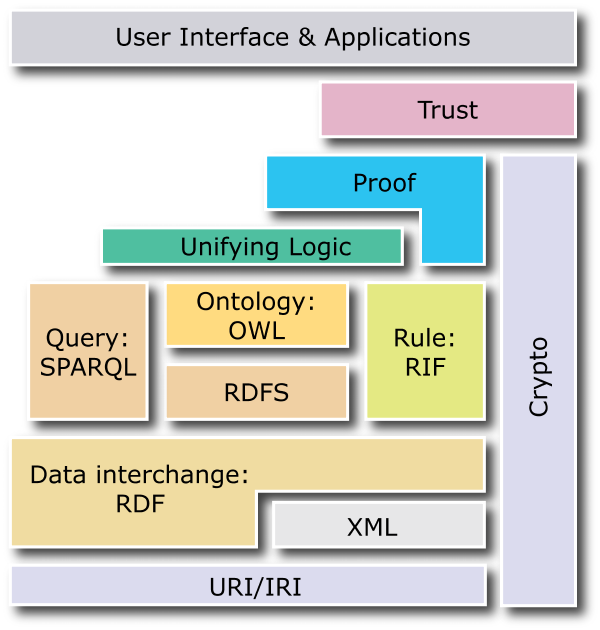
\includegraphics[width=160px]{Semantic_Web_Stack.png} 
 \end{figure}

 Il Web Semantico \`e costituito dall'insieme dei dataset 
 codificati ed esposti attraverso queste tecnologie.
\end{frame}

\begin{frame}
 \frametitle{Il protocollo SPARQL}
 Le basi di conoscenza presenti sul Web Semantico usualmente mettono 
 a disposizione uno \emph{SPARQL endpoint} che permette di interrogarle e,
 ove permesso, di modificarle.
 
 \begin{table}
 \begin{tabular}{|c|l|}
  \hline
  \bf{Knowledge Base} & \bf{Endpoint IRI} \\
  Europeana & \url{http://europeana.ontotext.com/sparql} \\
  CNR & \url{http://data.cnr.it/sparql/}\\
  Camera dei Deputati & \url{http://dati.camera.it/sparql}\\
  DBPedia & \url{http://dbpedia.org/sparql}\\
  \hline
 \end{tabular} 
 \caption{Alcuni endpoint sparql}
 \end{table}

\uncover<2->{
Il \emph{protocollo SPARQL} (vedi \url{http://www.w3.org/TR/sparql11-protocol/})
\`e basato sul protocollo HTTP le richieste SPARQL vengono inviate agli
endpoint come richieste GET o POST e l'endpoint risponde con un \emph{esito}.
\vspace{\baselineskip}
}

\uncover<3>{
Le richieste si suddividono in richieste di \emph{query} o \emph{update}.

In caso di richieste di tipo query effettuate con successo, la risposta alla
chiamata GET o POST conterr\`a anche tutte le \emph{soluzioni} dell'interrogazione
in uno dei formati XML, JSON o CSV (il formato di risposta va specificato 
nella richesta).
}
\end{frame}

\begin{frame}[fragile]
\frametitle{SPARQL Query Language}
Le richieste di tipo \emph{query} vanno specificate nel linguaggio
denominato \emph{SPARQL Query}.
%
La specifica di questo linguaggio \`e disponibile all'indirizzo
\begin{center}
 \url{http://www.w3.org/TR/sparql11-query/} .
\end{center}

Una \emph{query SPARQL} ha la seguente sintassi
\begin{Verbatim}[fontsize=\small]
BASE <iriBase>
PREFIX p1 : <iriP1>
...
PREFIX pn : <iriPn>

SELECT ?x1 ... ?xm WHERE { GraphPattern }
\end{Verbatim}
dove: 
\begin{itemize}
 \item la sezione $BASE\,<iriBase>$ \`e opzionale;
 \item $p1, \ldots, pn$ sono prefissi di namespace ($n\geq0$, se $n=0$ non \`e presente alcun prefisso);
 \item $<iriP1>, \ldots, <iriPn>$ sono IRI;
 \item $?x1, \ldots, ?xm$ sono \emph{variabili} ($m>0$);
 \item $GraphPattern$ \`e un \emph{graph pattern} di uno dei tipi che vedremo in seguito.
\end{itemize}
\end{frame}

\begin{frame}[fragile]
\frametitle{SPARQL Query Language - Triple Pattern}
Il tipo di graph pattern più basilare \`e quello dei \emph{triple pattern}.
Un triple pattern \`e una espressione di uno dei seguenti tipi:
\[
 s \, p \, o \,, \quad s \, \mathtt{a} \, o
\]
ove $s$ e $p$ possono essere IRI o variabili, \texttt{a} \`e una parola riservata, e $o$ pu\`o essere una
IRI, una variabile o un letterale.
\vspace{\baselineskip}

\uncover<2->{
  Le formule atomiche nelle query congiuntive possono essere facilmente tradotte in triple patterns:
  \begin{small}
  \[
    \begin{array}{lclr}
    C(?a) & \Longrightarrow & ?a\, \mathtt{a} \,C \quad | \quad ?a\, \mathtt{rdf:type}\, C \mbox{(le due formulazioni sono equivalenti)}\\    
    \\
    ?a\,P\,?b & \Longrightarrow & ?a\, P \,?b . 
    \end{array}
  \]
  \end{small}

  Si noti che la propriet\`a \texttt{rdf:type} viene utilizzata per esprimere l'appartenenza 
  nel linguaggio RDF.
\vspace{\baselineskip}
}

\uncover<3->{
  A differenza delle query congiuntive, in SPARQL le variabili possono comparire anche
  al posto del nome della classe o della propriet\`a. Ad esempio i seguenti due sono 
  triple pattern validi:
  
    \begin{small}
  \[
    \begin{array}{lr}
    ?C(a) & \mbox{``Trova tutte le classi cui appartiene }a\mbox{''}\\    
    \\
    ?a\,?p\,?b & \mbox{``Trova tutte le triple nell'ontologia''.}   
    \end{array}
  \]
  \end{small}
}
% Esempi di triple pattern sono
% 
% \begin{quote}
% ``Trova tutti gli individui maschi''
% \end{quote}
% \begin{Verbatim}[fontsize=\small]
% ?x rdf:type Male . 
% \end{Verbatim}
% 
% \begin{quote}
% ``Trova tutte le coppie [?x, ?y] in relazione \url{childOf}''
% \end{quote}
% \begin{Verbatim}[fontsize=\small]
% ?x childOf ?y . 
% \end{Verbatim}
\end{frame}

\begin{frame}[fragile]
\frametitle{SPARQL Query Language - Soluzioni}
Analogamente a quanto accade nell'ambito del conjunctive query answering,
le \emph{soluzioni} per un triple pattern $T$ rispetto a una ontologia $\Ont$ 
sono tutte le sostituzioni $\sigma$ che associano ad ogni variabile presente 
in $T$ una IRI o un letterale in modo tale che $\sigma T$ sia presente in $\Ont$.
\vspace{\baselineskip}

Il risultato di una query $Q$, avente come pattern un triple pattern $T$
e come variabili nella select $x_1, \ldots, x_n$,
rispetto all'ontologia $\Ont$ \`e l'insieme delle sostituzioni $\sigma$,
ristrette alle variabili $x_1, \ldots, x_n$, tali che
$\sigma T$ appartiene ad $\Ont$.
\end{frame}

\begin{frame}[fragile]
 \frametitle{SPARQL Query Language - Triple Pattern - Esempio}
 Consideriamo ad esempio la seguente ontologia (base prefix \url{http://ex.org/})
\begin{tabular}{cc}
$\begin{array}{cl}
  \Ont  =  &  \{Female(Elise), Female(Alice), Male(Bob), \\
  &\phantom{\{}Male(Charlie), Male(Daniel), \\
  &\phantom{\{}Alice\,childOf\,Elise, Charlie\,childOf\,Elise, \\
  &\phantom{\{}Daniel\,childOf\,Alice, Daniel\,childOf\,Bob, \\
  &\phantom{\{}Francis\,childOf\,Charlie \}
 \end{array}$ & 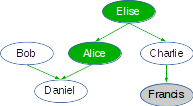
\includegraphics[width=120px]{family.png} \\
\end{tabular}

Consideriamo inoltre la query $Q$ definita come segue.

\begin{Verbatim}[fontsize=\small]
BASE <http://ex.org/>

SELECT ?x ?y WHERE { ?x childOf ?y . }
\end{Verbatim}

Le soluzioni di $Q$ rispetto a $\Ont$ sono
\begin{tabular}{|c|c|}
\hline 
?x & ?y \\
\hline
\url{<http://ex.org/Eliza>} & \url{<http://ex.org/Giorgia>} \\
\url{<http://ex.org/Eliza>} & \url{<http://ex.org/Francis>} \\
\hline 
\end{tabular}
\end{frame}

\begin{frame}[fragile]
 \frametitle{SPARQL Query Language - Basic Graph Pattern}
Un \emph{basic graph pattern} \`e un insieme di triple pattern, separati
dal carattere ``.''. Una sostituzione \`e una soluzione per un basic graph
pattern se e solo se \`e una soluzione per tutti i triple pattern
che compaiono in esso.
\vspace{\baselineskip}

Un esempio di query con il basic graph pattern \`e il seguente:
\begin{quote}
``Trova tutte le persone con almeno un figlo maschio''
\end{quote}
\begin{Verbatim}[fontsize=\small]
BASE <http://ex.org/>

SELECT ?x  WHERE { 
  ?y childOf ?x .
  ?y a Male
}
\end{Verbatim}
\vspace{\baselineskip}

\uncover<2->{
Da una query congiuntiva si pu\`o ottenere il basic graph pattern
corrispondente come segue:
\begin{itemize}
 \item applicare la trasformazione vista in precedenza ai triple pattern che lo costituiscono;
 \item sostituire i caratteri ``.'' con l'operatore logico di congiunzione $\wedge$.
\end{itemize}
Ad esempio
\[
 C(?x) \wedge ?x\,P\,b \quad \Longrightarrow \quad ?x\,\mathtt{a}\,C\,.\,?x\,P\,b\,.
\]
}
\end{frame}

\begin{frame}[fragile]
 \frametitle{SPARQL Query Language - Filtri sui letterali}
\`E possibile specificare dei filtri sui letterali che compaiono nei pattern.
Essi sono dei predicati, che dipendono dal tipo di dato dei letterali.\footnote{\url{http://www.w3.org/TR/sparql11-query/\#OperatorMapping}}
Permettono di selezionare tutte le soluzioni nelle quali ad una 
determinata variabile viene associato un letterale che soddisfa un predicato.
\vspace{\baselineskip}

La seguente query ad esempio permette di ottenere tutti
gli individui con un figlio il cui nome inizia con la lettera 'R'.
\begin{Verbatim}[fontsize=\small]
BASE <http://ex.org/>

SELECT ?x  WHERE { 
  ?y childOf ?x .
  ?y fullName ?name .
  FILTER regex(?name, "^R.*") .
}
\end{Verbatim}
\end{frame}

\begin{frame}[fragile]
 \frametitle{SPARQL Query Language - Optional Pattern Matching}

 Dati due graph pattern $P_1$ e $P_2$, il seguente \`e un \emph{optional graph pattern}:
\[
 P_1 \mathtt{OPTIONAL} P_2 .
\]

 Le sostituzioni che sono soluzioni per questo pattern sono quelle che
\begin{itemize}
 \item sono soluzioni per $P_1$ e $P_2$, oppure
 \item sono soluzioni per $P_1$
\end{itemize}
\end{frame}

\section{RDF}
\begin{frame}
 \frametitle{Resource Description Framework (RDF)}
 Il \emph{linguaggio di rappresentazione} pi\`u basilare nella pila
 delle tecnologie del Web Semantico \`e il cosiddetto 
 \emph{Resource Description Framework} (nel seguito \emph{RDF}).
 
  \begin{figure}
  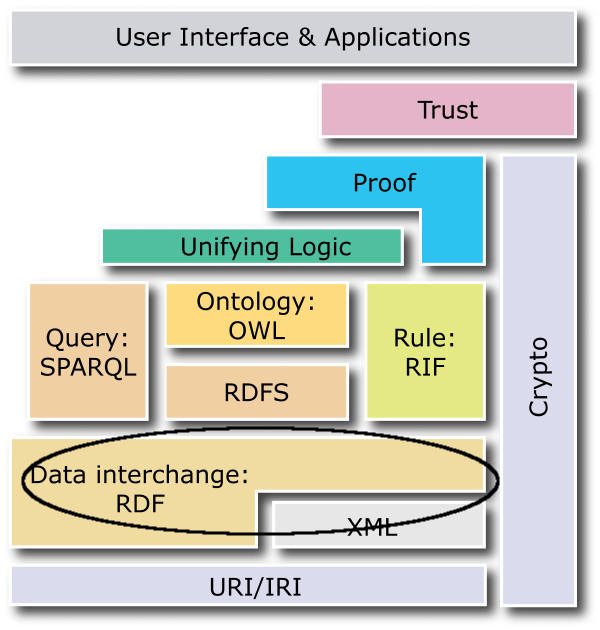
\includegraphics[width=160px]{Semantic_Web_Stack_RDF.png}
 \end{figure}
\end{frame}

\newcommand{\RDFv}{\mathtt{RDF}}

\begin{frame}
 \frametitle{Grafi RDF}
 Le ontologie RDF sono dette \emph{grafi RDF} in quanto possono contenere solo
 property assertions.
 \vspace{\baselineskip}
 
 \uncover<2->{ 
 Un \emph{grafo RDF} \`e un insieme finito di property assertions dei seguenti tipi:
\[
 \begin{array}{rcl}
  a & P & b \\
  a & P & l
 \end{array}
\]
con 
\[
 \begin{array}{l}
 P \in \IRI\\
 a, b \in \IRI \cup \BlankNodes\\
 l \in \literals
 \end{array}
\]
per qualche insieme $\BlankNodes$ disgiunto da $\IRI$.
\vspace{\baselineskip}
}

\uncover<3->{
Dato un grafo RDf $G$, gli elementi di $\BlankNodes$ che compaiono in $G$ sono
definiti \emph{blank node} di $G$. Indicheremo con
$\BlankNodes(G)$ l'insieme dei blank node del grafo $G$.
}
\end{frame}

\newcommand{\triple}[3]{\mathurl{#1}\;\mathurl{#2}\;#3}
\newcommand{\tripleO}[3]{\mathurl{#1}\;\mathurl{#2}\;\mathurl{#3}}

\begin{frame}
 \frametitle{Grafi RDF - Esempio}
 Un esempio di grafo RDF \`e il seguente:
 \[
 \begin{array}{rcl}
  G & \defAs & \{ \tripleO{ex:Alice}{ex:childOf}{ex:Eliza},\\
  &&\phantom{\{} \tripleO{ex:Bob}{ex:childOf}{ex:Eliza},\\
  &&\phantom{\{} \triple{ex:Eliza}{ex:fullName}{\stringLiteral{Eliza Smith}},\\
  &&\phantom{\{} \triple{ex:Eliza}{ex:age}{\literal{63}{xsd:nonNegativeInteger}} \,\},\\
 \end{array}
\]
\end{frame}

\begin{frame}
 \frametitle{RDF - Semantica}
 Esistono alcuni nomi di propriet\`a, di classi e di individui che ricoprono
 dei ruoli \emph{particolari} nel linguaggio RDF:

 \[
 \begin{array}{lc}
	\mathurl{rdf:Property}, \mathurl{rdf:List} & \in \CNames; \\ 
	\mathurl{rdf:type}, \mathurl{rdf:subject}, \mathurl{rdf:predicate},
 	\mathurl{rdf:object}, \\
 	&\\
	\mathurl{rdf:first}, \mathurl{rdf:rest}, \mathurl{rdf:value}, \mathurl{rdf:_1},
 	 \mathurl{rdf:_2}, \ldots & \in \PNames ;\\
 	&\\  
	\mathurl{rdf:nil} & \in \INames; \\
	&\\
	\mathurl{rdf:XMLLiteral} & \in \DNames.
\end{array}
 \]
	dove il prefisso \url{rdf:} \`e una abbreviazione per il namespace
	\begin{center}
	\url{http://www.w3.org/1999/02/22-rdf-syntax-ns\#}
	\end{center}
	\vspace{\baselineskip}
 
 Una \emph{interpretazione RDF} pone dei vincoli semantici particolari
 sull'interpretazione di questi termini (ne vedremo solo alcuni).
\end{frame}

\begin{frame}
 \frametitle{Class assertions in RDF}
 Asserzioni del tipo $a\, \mathurl{rdf:type}\,C$ vengono usate in RDF 
 per affermare class assertions $C(a)$.
 \[
 \I \models a\; \mathurl{rdf:type}\;C \Leftrightarrow C^{\I}(a^{\I}) \quad (*)
 \]

\uncover<2->{  
 In altre parole, da ogni asserzione del tipo $a\, \mathurl{rdf:type}\,C$
 tramite reasoning viene inferita una asserzione $C(a)$.
 \vspace{\baselineskip}
 
 Ad esempio:
 \[
 \begin{small}
 \begin{array}{lcl}
  \{ \tripleO{ex:Eliza}{rdf:type}{ex:Person},&&\{ \mathurl{ex:Person}(\mathurl{ex:Eliza}),\\
  \phantom{\{} \tripleO{ex:Alice}{rdf:type}{ex:Person},&&\phantom{\{}\mathurl{ex:Person}(\mathurl{ex:Alice}),\\
  \phantom{\{} \tripleO{ex:Bob}{rdf:type}{ex:Person},&&\phantom{\{}\mathurl{ex:Person}(\mathurl{ex:Bob}),\\
  \phantom{\{} \tripleO{ex:childOf}{rdf:type}{rdf:Property},& \Longrightarrow & \phantom{\{}\mathurl{ex:Property}(\mathurl{ex:childOf}),\\
  \phantom{\{} \tripleO{ex:fullName}{rdf:type}{rdf:Property},&&\phantom{\{}\mathurl{ex:Property}(\mathurl{ex:fullName}),\\
  \phantom{\{} \tripleO{ex:age}{rdf:type}{rdf:Property},&&\phantom{\{}\mathurl{ex:Property}(\mathurl{ex:age}),\}\\
  \phantom{\{} \tripleO{ex:Alice}{ex:childOf}{ex:Eliza},&&\phantom{\{}\ldots \, \}\\
  \phantom{\{} \tripleO{ex:Bob}{ex:childOf}{ex:Eliza},\\
  \phantom{\{} \triple{ex:Eliza}{ex:fullName}{\stringLiteral{Eliza Smith}},\\
  \phantom{\{} \triple{ex:Eliza}{ex:age}{\literal{63}{xsd:nonNegativeInteger}} \,\},\\
\end{array}
\end{small}
\]
}
\end{frame}

\begin{frame}
 \frametitle{La classe \url{rdf:Property}}
Ogni propriet\`a $P$ presente in un grafo RDF deve essere una
istanza della classe \url{rdf:Property} 
\[
  \I \models a\,P\,b \iff [a^{\I}, b^{\I}] \in P^{\I} \wedge P^{\I} \in
  (\mathurl{rdf:Property})^{\I} \quad (**).
\]

\uncover<2>{
Supponiamo che la seguente asserzione sia in un grafo RDF $G$ e sia
$G'$ l'ontologia delle asserzioni che \`e possibile inferire da $G$ 
\[
 \tripleO{ex:Bob}{ex:childOf}{ex:Eliza} .
\]
Allora
\[
 \begin{array}{ll}
 \tripleO{ex:Bob}{ex:childOf}{ex:Eliza} \in G & \Longrightarrow (**)\\
 \mathurl{rdf:Property}(\mathurl{ex:childOf}) \in G' & \Longrightarrow (*) \\
 \tripleO{ex:childOf}{rdf:type}{rdf:Property} \in G'\\
 \end{array}
\]
}
\end{frame} 

\begin{frame}
 \frametitle{Propriet\`a e Class in RDF}
 Si noti che le propriet\`a e le classi in RDF sono trattate anche come
 \emph{individui}. In altre parole, nel contesto RDF
 \[
 \begin{array}{c}
  \PNames \subseteq \INames ,\\
  \\
  \mathurl{rdf:Property} \in \CNames \cap \INames . 
 \end{array}
 \]
 \vspace{\baselineskip}
 
 Operazioni di questo tipo sono in genere \emph{rischiose} in termini 
 di indecidibilit\`a (vedi OWL Full).   
 \vspace{\baselineskip}

 In genere, la natura di individuo di una propriet\`a classi viene
 utilizzata solo  per \emph{annotare} le propriet\`a con commenti ed etichette
 esplicative oppure per descrivere i vincoli, come vedremo più avanti.
\end{frame} 

% \section{Serializzazioni}
% 
\begin{frame}
 \frametitle{Serializzazione di grafi RDF}
 
 Il processo di serializzazione di un grafo RDF permette
 di scrivere un grafo su un file o di inviarlo in rete.
 \vspace{\baselineskip}
 
 La serializzazione di un grafo RDF genera una stringa di testo
 in una delle seguenti \emph{sintassi concrete}:
 \begin{itemize}
  \item NTriples
  \item Turle
  \item RDF XML
  \item RDFa
  \item ...
 \end{itemize}
\end{frame} 

\begin{frame}[fragile]
 \frametitle{La Sintassi RDF N-Triples}
 
 Un grafo RDF serializzato secondo la sintassi N-Triples \`e
 una sequenza di righe con la seguente sintassi
\[
\begin{array}{rcl}
 r & := & <IRI> \quad <IRI> \quad o . \\
 o & := & <IRI> | \stringLiteral{STRING} | \literal{STRING}{<IRI>}
\end{array} 
\]
dove $IRI$ sono delle IRI e $STRING$ stringhe UNICODE.
\vspace{\baselineskip}

Intuitivamente, ogni riga di un file N-Triples rappresenta 
una property assertion RDF. Nel seguito un esempio di grafo
RDF espresso in N-Triples.
\vspace{\baselineskip}


\begin{Verbatim}[fontsize=\small]
<http://ex.org/Alice> <http://ex.org/childOf> <http://ex.org/Eliza> .
<http://ex.org/Bob> <http://ex.org/childOf> <http://ex.org/Eliza> .
<http://ex.org/Bob> <http://ex.org/childOf> <http://ex.org/Eliza> .
<http://ex.org/Eliza> <http://ex.org/fullName> "Eliza Smith" .
<http://ex.org/Eliza> <http://ex.org/age> 
                        "63"^^<http://www.w3.org/2001/XMLSchema#nonNegativeInteger> .
\end{Verbatim}
\end{frame}

\begin{frame}[fragile]
 \frametitle{La Sintassi RDF Turle - Predicate List}
 
\emph{Turtle} estende N-Triples con alcune funzionalit\`a.
\vspace{\baselineskip}

\emph{Predicate List} - Usando il simbolo ``;'' al posto di ``.'' al termine di alcune righe \`e possibile
specificare coppie [predicato, oggetto] che si riferiscono allo stesso soggetto. Ad esempio, le seguenti
righe (N-Triples)

\begin{Verbatim}[fontsize=\small]
<http://ex.org/Eliza> <http://ex.org/childOf> <http://ex.org/Giorgia> .
<http://ex.org/Eliza> <http://ex.org/childOf> <http://ex.org/Francis> .
<http://ex.org/Eliza> <http://ex.org/fullName> "Eliza Smith" .
<http://ex.org/Eliza> <http://ex.org/age> 
                        "63"^^<http://www.w3.org/2001/XMLSchema#nonNegativeInteger> .
\end{Verbatim}

possono essere espresse in Turtle come segue:
\begin{Verbatim}[fontsize=\small]
<http://ex.org/Eliza> <http://ex.org/childOf> <http://ex.org/Giorgia> ;
                      <http://ex.org/childOf> <http://ex.org/Francis> ;
                      <http://ex.org/fullName> "Eliza Smith" ;
                      <http://ex.org/age> 
                         "63"^^<http://www.w3.org/2001/XMLSchema#nonNegativeInteger> .
\end{Verbatim}
\end{frame}

\begin{frame}[fragile]
 \frametitle{La Sintassi RDF Turle - Object List}
Analogamente, usando simbolo ``,'' al posto di ``.'' al termine di alcune righe \`e possibile
specificare molteplici \emph{oggetti} che si riferiscono alla stessa coppia [soggetto, predicato]
Ad esempio

\begin{Verbatim}[fontsize=\small]
<http://ex.org/Eliza> <http://ex.org/childOf> <http://ex.org/Giorgia> .
<http://ex.org/Eliza> <http://ex.org/childOf> <http://ex.org/Francis> .
\end{Verbatim}

possono essere abbreviate con
\begin{Verbatim}[fontsize=\small]
<http://ex.org/Eliza> <http://ex.org/childOf> <http://ex.org/Giorgia> ,
                                              <http://ex.org/Francis> .
\end{Verbatim}
\end{frame}
 
\begin{frame}[fragile]
 \frametitle{La Sintassi RDF Turle - Prefisso base}

Con la parola chiave base \`e possibile specificare un \emph{prefisso base}
che verr\`a utilizzato per risolvere le IRI incomplete presenti nel grafo RDF.

\begin{Verbatim}[fontsize=\small]
BASE <http://ex.org/> .

<Eliza> <childOf>  <Giorgia> ,
                   <Francis> .
<Eliza> <fullName> "Eliza Smith" ;
        <age> "63"^^<http://www.w3.org/2001/XMLSchema#nonNegativeInteger> .
\end{Verbatim}
\end{frame}

\begin{frame}[fragile]
 \frametitle{La Sintassi RDF Turle - Prefissi}

\`E possibile inoltre dichiarare anche altri \emph{prefissi} da utilizzare
per abbreviare le IRI.

\begin{Verbatim}[fontsize=\small]
BASE <http://ex.org/>
PREFIX rdf: <http://www.w3.org/1999/02/22-rdf-syntax-ns#>
PREFIX xsd: <http://www.w3.org/2001/XMLSchema#> .

<Eliza>   <rdf:type> <Person> .
<Giorgia> <rdf:type> <Person> .
<Francis> <rdf:type> <Person> .
<Eliza>   <childOf>  <Giorgia> ,
                     <Francis> . 
<Eliza>   <fullName> "Eliza Smith" ;
          <age>      "63"^^<xsd:nonNegativeInteger> .
\end{Verbatim}
\end{frame}

\begin{frame}[fragile]
 \frametitle{La Sintassi RDF Turle - \url{rdf:type}}

Il simbolo 'a' pu\`o essere usato al posto del predicato \url{rdf:type}.

\begin{Verbatim}[fontsize=\small]
BASE <http://ex.org/> .
PREFIX rdf: <http://www.w3.org/1999/02/22-rdf-syntax-ns#> .
PREFIX xsd: <http://www.w3.org/2001/XMLSchema#> .

<Eliza> a <Person> .
<Giorgia> a <Person> .
<Francis> a <Person> .
<Eliza> <childOf> <Giorgia> ,
                  <Francis> .
<Eliza>  <fullName> "Eliza Smith" ;
         <age> "63"^^<xsd:nonNegativeInteger> .
\end{Verbatim}
\end{frame}

\begin{frame}[fragile]
 \frametitle{La Sintassi RDF Turle - Letterali}

Turtle definisce alcune abbreviazioni anche per i letterali,
che permettono di non indicare esplicitamente il data type.
Ad esempio:

\begin{Verbatim}[fontsize=\small]
BASE <http://ex.org/>

<http://en.wikipedia.org/wiki/Helium>                                                                                  
    :atomicNumber 2 ;               # xsd:integer                                                                      
    :atomicMass 4.002602 ;          # xsd:decimal                                                                      
    :specificGravity 1.663E-4 .     # xsd:double   
\end{Verbatim}
\vspace{\baselineskip}

Per un elenco completo delle abbreviazioni disponibili in Turtle per i
letterali fare riferimento a \url{http://www.w3.org/TR/2014/REC-turtle-20140225/\#literals} .
\end{frame}

\begin{frame}
 \frametitle{La Sintassi RDF XML}
 La sintassi \emph{RDF XML} permette di serializzare un grafo RDF 
 in un documento XML. L'elemento radice di questo documento \`e di
 tipo \url{rdf:RDF}.
 \vspace{\baselineskip}
 
 Gli elementi figli della radice sono di tipo \url{rdf:Description}
 e rappresentano \emph{nodi} del grafo RDF (individui). La IRI associata 
 al nodo viene specificata con l'attributo \url{rdf:about}. Nel caso in
 cui non sia presente l'attributo \url{rdf:about} siamo in presenza
 di un blank node.
 \vspace{\baselineskip}

 I figli di ogni elemento di tipo \url{rdf:Description} sono le
 propriet\`a con le quali sono etichettati gli archi uscenti dal 
 nodo che stiamo rappresentando.
 \vspace{\baselineskip}

 A loro volta, tali elementi rappresentanti gli archi uscenti da
 un nodo possono avere come figli 
 \begin{itemize}
  \item altri elementi di tipo \url{rdf:Description}, nel caso in cui
  l'oggetto della asserzione sia un individuo,
  \item degli elementi con un datatype come tipo, nel caso in cui 
  l'oggetto della asserzione sia un letterale,
  \item oppure possono avere un attributo \url{rdf:resource} che ha
  come valore la IRI associata all'individuo oggetto dell'asserzione.
 \end{itemize}
\end{frame}

\begin{frame}[fragile]
 \frametitle{La Sintassi RDF XML - Property assertions}
 In altre parole, una property assertion del tipo $\tripleO{iriSubj}{iriProp}{iriObj}$,
 con $iriSubj, iriProp, iriObj \in \IRI$ pu\`o essere serializzata in RDF XML 
 con il seguente elemento 

 \begin{Verbatim}[fontsize=\small]
   <rdf:Description rdf:about="iriSubj">
     <iriProp>
       <rdf:Description rdf:about="iriObj" />
     <iriProp>      
   </rdf:Description>
\end{Verbatim}

oppure, utilizzando \url{rdf:resource}, con

\begin{Verbatim}[fontsize=\small]
   <rdf:Description rdf:about="iriSubj">
     <iriProp rdf:resource="iriObj" />
   </rdf:Description>
\end{Verbatim}
\end{frame}

\begin{frame}[fragile]
 \frametitle{La Sintassi RDF XML - Multiple Property assertions}
 
 
 Inoltre, property assertions con lo stesso oggetto possono essere 
 raggruppate all'interno di un unico elemento di tipo \url{rdf:Description}.
 Vediamo ad esempio una possibile serializzazione in RDF XML di due asserzioni 
 con lo stesso soggetto.
\[
\begin{array}{l}
 iriSubj\,iriProp1\,iriObj1 \,, \\
 iriSubj\,iriProp2\,iriObj2
\end{array}
\]

\begin{Verbatim}[fontsize=\small]
   <rdf:Description rdf:about="iriSubj">
     <iriProp1 rdf:resource="iriObj1" />
     <iriProp2 rdf:resource="iriObj1" />
   </rdf:Description>
\end{Verbatim}
\end{frame}

\begin{frame}[fragile]
 \frametitle{La Sintassi RDF XML - String literals}
I letterali di tipo stringa specificati come oggetto di una 
properti assertions vanno inseriti come contenuto (CDATA) dell'elemento
che identifica la propriet\`a all'interno degli elementi \url{rdf:Description}.

Ad esempio una asserzione del tipo seguente
\[
 \triple{iriSubj}{iriProp}{\stringLiteral{string}}
\]
pu\`o essere serializzata come segue:
\vspace{\baselineskip}

\begin{Verbatim}[fontsize=\small]
   <rdf:Description rdf:about="iriSubj">
     <iriProp>string</iriProp>
   </rdf:Description>
\end{Verbatim}
\end{frame}

\begin{frame}[fragile]
 \frametitle{La Sintassi RDF XML - Datatype property}
\`E possibile inoltre specificare esplicitamente il datatype di un
letterale oggetto di una property assertion mediante l'attributo \url{rdf:datatype}.

\[
 \triple{iriSubj}{iriProp}{\literal{lexForm}{iriType}}
\]
\vspace{\baselineskip}

\begin{Verbatim}[fontsize=\small]
   <rdf:Description rdf:about="iriSubj">
     <iriProp rdf:datatype="iriType">lexForm</iriProp>
   </rdf:Description>
\end{Verbatim}
\end{frame}

\begin{frame}[fragile]
 \frametitle{La Sintassi RDF XML - Namespace}
Le abbreviazioni per i prefissi possono essere implementate attraverso
i meccanismi forniti dalla specifica XML. Segue un esempio completo
di grafo RDF serializzato in RDF/XML.
\vspace{\baselineskip}

\begin{Verbatim}[fontsize=\small]
<?xml version="1.0"?>
<rdf:RDF xmlns="http://ex.org/"
  xmlns:rdf="http://www.w3.org/1999/02/22-rdf-syntax-ns#"
  xmlns:xsd="http://www.w3.org/2001/XMLSchema#">

  <rdf:Description rdf:about="Giorgia">
    <rdf:type rdf:resource="http://ex.org/Person" />
  </rdf:Description>

  <rdf:Description rdf:about="Francis">
    <rdf:type rdf:resource="http://ex.org/Person" />
  </rdf:Description>
  
  <rdf:Description rdf:about="Eliza">
    <rdf:type rdf:resource="http://ex.org/Person" />
    <childOf>
      <rdf:Description rdf:about="Giorgia" />
      <rdf:Description rdf:about="Francis" />
    </childOf>    
    <fullName>Eliza Smith</fullName>
    <age rdf:datatype="http://www.w3.org/2001/XMLSchema#nonNegativeInteger">63</age>
  </rdf:Description>
</rdf:RDF>
\end{Verbatim}
\end{frame}

\begin{frame}[fragile]
 \frametitle{La Sintassi RDF XML - Typed Node Elements}
 
Se un individuo appartiene ad una classe con  
una qualche IRI $uriClass$, ossia se una una tripla del 
tipo
\[
 uriInd\,\mathurl{rdf:type}\,uriClass
\]
compare nel grafo RDF, \`e possibile non usare \url{rdf:Description}
per indicare l'individuo $uriInd$, ma al suo posto dichiarare
nel documento XML un elemento di tipo $uriClass$.
\vspace{\baselineskip}

Ad esempio, e seguenti due serializzazioni sono equivalenti.

\begin{Verbatim}[fontsize=\small]
  <rdf:Description rdf:about="Eliza">
    <rdf:type rdf:resource="http://ex.org/Person" />
    <childOf rdf:resource="http://ex.org/Giorgia" />
    <childOf rdf:resource="http://ex.org/Francis" />
    <fullName>Eliza Smith</fullName>
    <age rdf:datatype="http://www.w3.org/2001/XMLSchema#nonNegativeInteger">63</age>
  </rdf:Description>
\end{Verbatim}

\begin{Verbatim}[fontsize=\small]
  <Person rdf:about="Eliza">
    <childOf rdf:resource="http://ex.org/Giorgia" />
    <childOf rdf:resource="http://ex.org/Francis" />
    <fullName>Eliza Smith</fullName>
    <age rdf:datatype="http://www.w3.org/2001/XMLSchema#nonNegativeInteger">63</age>
  </Person>
\end{Verbatim}
\end{frame}

\begin{frame}
 \frametitle{RDF Schema}
 \emph{RDF Schema} (in breve \emph{RDFS}) estende RDF con 
 ulteriori classi e propriet\`a per descrivere \emph{vincoli semantici}.
 \vspace{\baselineskip}
 
 In questa sede vedremo $\mathurl{rdfs:Class} \in \CNames$ e le propriet\`a 
 $\mathurl{rdfs:subClassOf}$, $\mathurl{rdfs:subPropertyOf}$,
 $\mathurl{rdfs:domain}$, $\mathurl{rdfs:range}$, $\mathurl{rdfs:label}$,
 $\mathurl{rdfs:comment}$ dove il prefisso \url{rdfs} \`e una abbreviazione per
 il namespace
\begin{center}
 \url{http://www.w3.org/2000/01/rdf-schema\#}
\end{center}
\end{frame}

\begin{frame}
 \frametitle{Classi RDFS}
 In RDFS \`e definita una classr \url{rdfs:Class} cui appartengono tutte le
 altre classi:
\[
\begin{array}{lcl}
	C \in \CNames \Longrightarrow C^{\I} \in  (\mathurl{rdfs:Class})^{\I}\\
\end{array}
\]
per ogni interpretazione RDFS $\I$. 
\end{frame}

\begin{frame}
 \frametitle{Gerarchie di Classi e Propriet\`a}
 In RDFS \`e possibile definire gerarchie di classi.

\[
\begin{array}{lcl}
	\I \models C\;\mathurl{rdfs:subClassOf}\;D & \iff & \I \models C \Issub D\\
	&&\\
	\I \models P\;\mathurl{rdfs:subPropertyOf}\;Q & \iff & \I \models P \Issub Q\\
\end{array}
\]
per ogni $C, D \in \CNames$, $P, Q \in \PNames$ e per ogni interpretazione RDFS
$\I$.
\end{frame}

\begin{frame}
 \frametitle{Vincoli di Dominio e Codominio}
 Si possono esprimere restrizioni sul dominio e codominio di una proprietà
\[
\begin{array}{lcl}
	\I \models P\;\mathurl{rdfs:domain}\;C & \iff & \I \models \dom(P) \Issub C\\
	&&\\
	\I \models P\;\mathurl{rdfs:range}C & \iff & \I \models \range(P) \Issub C\\
\end{array}
\]
per ogni $C \in \CNames$, $P \in \PNames$ e per ogni interpretazione RDFS
$\I$.
\end{frame}

\begin{frame}[fragile]
 \frametitle{Annotazioni}
 \`E inoltre possibile \emph{annotare} classi e propriet\`a con 
 delle descrizioni intuitive.
 \vspace{\baselineskip}
 
\begin{Verbatim}[fontsize=\small]
<rdfs:Class rdf:about="http://ex.org/Man">
  <rdfs:subClassOf rdf:resource="http://ex.org/Person" />
  <rdfs:label>Man</rdfs:label>
  <rdfs:comment>A male person.</rdfs:comment>
</rdf:Class>
\end{Verbatim} 
\end{frame}

\section{Vocabolari}

\begin{frame}
\frametitle{Vocabolari}
	
	Nomi di classe e propriet\`a vengono raggruppati in \emph{vocabolari}
	che trattano specifici domini di conoscenza (eg. organizzazioni, 
	pubblica amministrazione, biologia, commercio, etc.). 
	\vspace{\baselineskip}
	
	Un vocabolario
	pu\`o contenere anche \emph{vincoli} inerenti classi e le propriet\`a 
	del vocabolario stesso.
	\vspace{\baselineskip}
	
	L'utilizzo di vocabolari condivisi permette lo sviluppo di applicazioni
	riguardanti specifici domini di conoscenza, ma indipendenti dai dati
	e dai dataset.
\end{frame}

\begin{frame}
\frametitle{Definizione di Vocabolario}
	Una definizione di vocabolario pu\`o essere la seguente:
	\[
	 V = (C, P, \Omega)
	\]
	dove
	\begin{enumerate}
	 \item $C$ \`e un sottoinsieme finito di $\CNames$,
	 \item $P$ \`e un sottoinsieme finito di $\PNames$,
	 \item $\Omega$ \`e un insieme finito di vincoli che coinvolgano solo
	 nomi di classi in $C$ e nomi di propriet\`a in $P$.
	\end{enumerate}
\end{frame}

\begin{frame}
  \frametitle{Il Vocabolario FOAF}
  Uno dei primi e pi\`u utilizzati vocabolari definiti nell'ambito
  del Web semantico \`e \emph{Friend OF A Friend} (\emph{FOAF}, vedi \url{http://foaf-project.org}).
  \vspace{\baselineskip}

  \begin{quote}
  FOAF is a project devoted to linking people and information using the Web. 
  \end{quote}
  \vspace{\baselineskip}

  Il vocabolario \`e disponibile alla URL
  \begin{center}
    http://xmlns.com/foaf/spec/index.rdf  
  \end{center}
  \vspace{\baselineskip}

  Il namespace del vocabolario FOAF \`e \url{http://xmlns.com/foaf/0.1/}
  \vspace{\baselineskip}
  
  \texttt{foaf-a-matic}\footnote{\url{http://www.ldodds.com/foaf/foaf-a-matic.html}} \`e uno strumento \emph{giocattolo} che permette di realizzare facilmente
  una ontologia che usa il vocabolario FOAF.
\end{frame}

\newcommand{\foafcore}{\mathtt{FOAFCore}}
\begin{frame}
  \frametitle{FOAF Core}

  In questa sede ci limiteremo solo alla parte \emph{Core}.
  \vspace{\baselineskip}
  
  Il vocabolario \emph{Foaf Core} \`e definito come segue:
\[
 \begin{array}{ccl}
 \foafcore & \defAs & (C_{foaf}, P_{foaf}, \Omega_{foaf}) \\
 &&\\
 C_{foaf} & \defAs & \{Agent, Person, Project, Organization, Group, Document, Image\}\\
 &&\\
 P_{foaf} & \defAs & \{name, title, img, depiction, depicts, familyName, givenName, knows,\\
 && \phantom{\}} based\_near, age, made, maker, primaryTopic, primaryTopicOf, member \}\\
 \Omega_{foaf} & \defAs & \{ Person \Issub Agent, Group \Issub Agent, Organization \Issub Agent, \\
 && \phantom{\{} Image \Issub Document, \dom(title) \Issub Document, \\
 && \phantom{\{}\range(depiction) \Issub Image, img \Issub depiction, \dom(img) \Issub Person,\\
 && \phantom{\{}\dom(knows) \Issub Person, \range(knows) \Issub Person, \ldots \}\\
 \end{array}
\]
\end{frame}


\begin{frame}
  \frametitle{FOAF Core - classi}
  Nel seguito lasceremo ometteremo il prefisso delle URI, dando per scontato che sia 
  quello del vocabolario FOAF.
  \vspace{\baselineskip}
  
  Nel \emph{core} del vocabolario FOAF vengono definte le seguenti classi:
  
  \begin{itemize}
   \item \emph{Agent} - appartengono a questa classe tutte quelle entit\`a in grado di compiere azioni
   (persone, gruppi, software, robot, ...);   
   \item \emph{Person} ($Person \Issub Agent$) - persone (vive o morte, reali o immaginarie);
   \item \emph{Group} ($Group \Issub Agent$) - insiemi di agenti;
   \item \emph{Organization} ($Organization \Issub Agent$) - insiemi di persone che rappresenta una \emph{istituzione sociale} (azienda, associazione, ministero, ...);
   \item \emph{Document} sono i documenti, nel senso comune del termine (atti, leggi, carte di identit\`a, ...);
   \item \emph{Image} - ($Image \Issub Document$) - i documenti che sono immagini, sia digitali che non;
   \item \emph{Project} - un incontro collettivo di qualche tipo.
  \end{itemize}
\end{frame}

\begin{frame}
  \frametitle{FOAF Core - Propriet\`a}
  Elenchiamo ora le propriet\`a nel FOAF Core:
  
  \begin{itemize}
%    \item \emph{homepage} ($\range(homepage) \Issub Document$) - la pagina principale che descrive qualcosa;
   \item \emph{name} - il nome di qualcosa;
   \item \emph{title} - titolo onorifico di una person (Mr, Mrs, Ms, Dr. etc);
   \item \emph{familyName} ($\dom(familyName) \Issub Person$) - il cognome di una persona;
   \item \emph{givenName} - prima parte del nome completo di una persona;
   \item \emph{img} ($\dom(img) \Issub Person$, $\range(img) \Issub Image$) - mette in relazione una persona con 
   una immagine che la rappresenta;
   \item \emph{based\_near} ($\dom(based\_near) \Issub Spatial_Thing$, $\range(based_near) \Issub Spatial_Thing$) - 
    indica che due cose sono \emph{vicine} in termini spaziali;
   \item \emph{age} ($\dom(age) \Issub Agent$) - l'et\`a, espressa in numero di anni, di un agente;    
   \item \emph{knows} ($\dom(knows) \Issub Person$, $\range(knows) \Issub Person$) - indica che \`e avvenuta interazione
   di qualche tipo tra due persone;
   \item \emph{primaryTopicOf} ($\dom(primaryTopicOf) \Issub Document$) - indica l'oggetto principale di un documento;
   \item \emph{isPrimaryTopicOf} ($\range(isPrimaryTopicOf) \Issub Document$) - mette in relazione un oggetto con i 
    documenti che lo rigurdano;
   \item \emph{made} ($\dom(made) \Issub Agent$) - mette in relazione un agente con qualcosa 
   che ha prodotto;
   \item \emph{maker} ($\range(made) \Issub Agent$) - mette in relazione un oggetto con gli agenti
   che hanno contribuito a crearlo; 
   \item \emph{member} ($\dom(member) \Issub Group$, $\range(member) \Issub Agent$) - mette in relazione un
   gruppo con i suoi membri.
  \end{itemize}
\end{frame}

\begin{frame}
\frametitle{Descrizioni Intuitive degli Elementi dei Vocabolari}
	Le classi e le propriet\`a di un vocabolario vengono spesso fornite
	di una descrizione intuitiva nel documento che descrive il vocabolario.
	Ad esempio, le classi $Agent$ e $Person$ vengono descritte come segue
	in \url{http://xmlns.com/foaf/spec/}
	\begin{quote}
		\textbf{Agent} - The Agent class is the class of agents; things that do stuff. A well known
		sub-class is Person, representing people. Other kinds of agents include
		Organization and Group.
		
		The Agent class is useful in a few places in FOAF where Person would have
		been overly specific. For example, the IM chat ID properties such as
		jabberID are typically associated with people, but sometimes belong to
		software bots.
	\end{quote}

	\begin{quote}
		\textbf{Person} - The Person class represents people. Something is a Person if it is a person.
		We don't nitpic about whether they're alive, dead, real, or imaginary.
		The Person class is a sub-class of the Agent class, since all people are
		considered 'agents' in FOAF.
	\end{quote}
\end{frame}

\begin{frame}
\frametitle{Descrizioni Rigorose degli Elementi dei Vocabolari}
	Tuttavia, gi\`a nei vincoli di un vocabolario si trovano indicazioni importanti
	sulla \emph{semantica} dei nomi di classe e di propriet\`a del vocabolario stesso.
	\[
	\begin{array}{l}
	Person \Issub Agent\\
	\range(depiction) \Issub Image\\
	img \Issub depiction, \\
	\dom(img) \Issub Person,\\
	\dom(knows) \Issub Person,\\
	\range(knows) \Issub Person,\\
	\ldots
	\end{array}
	\]
\end{frame}
\end{document}
